\documentclass[11pt,a4paper]{article}
\usepackage[T1]{fontenc}
\usepackage[utf8]{inputenc}
\usepackage[french]{babel}
\usepackage{geometry}
\usepackage{graphicx}
\usepackage{booktabs}
\usepackage{listings}
\usepackage{hyperref}
\usepackage{float}
\usepackage{longtable}

\geometry{margin=2.2cm}
\setlength{\emergencystretch}{2em}
\hypersetup{colorlinks=true,linkcolor=blue,urlcolor=blue}

\lstset{basicstyle=\ttfamily\small,breaklines=true,frame=single,language=C++}

\title{Rapport technique, Lab 3\\
\large Contrôleur d'admission sur la zone dense Wi-Fi\\
Dépôt \texttt{ns3\_IMT2030\_connectivity}}
\author{Traorehub, travail de recherche en cours}
\date{Novembre 2026}

\begin{document}
\maketitle
\tableofcontents
\newpage

\section{Objectif du laboratoire}

Le Lab 2 a comparé les politiques \texttt{baseline} et \texttt{adaptive} sur un plan de 24 runs. Le contrôleur n'a modifié les octets reçus dans aucune cellule. Il est resté inactif sur 23 cellules, et les 50 événements enregistrés à 100 terminaux et 40~ms n'ont pas changé la livraison. Le Lab 3 reprend le même plan factoriel avec un émetteur et une loi d'admission qui agissent sur les paquets réellement émis.

La question de recherche est la suivante. Une admission permanente, calibrée sur une capacité de référence, élève-t-elle le taux de livraison des octets émis, et que devient le volume reçu par le point d'accès ? Le modèle radio reste le proxy Wi-Fi 802.11n des labs précédents, avec Yans, le débit \texttt{HtMcs7} et le SSID \texttt{imt2030-dense-zone}. La grille demeure une zone représentative. Elle ne simule pas un kilomètre carré peuplé d'un nœud par équipement.

\section{Pourquoi le contrôleur du Lab 2 n'agissait pas sur le trafic}

La version du Lab 2 s'appuyait sur \texttt{UdpClient}. Le contrôleur appelait \texttt{Stop}, puis \texttt{Start}, sur le conteneur d'applications. Ces méthodes écrivent les dates de début et de fin de l'application. Après l'initialisation, elles n'annulent pas l'événement \texttt{m\_sendEvent} déjà planifié dans \texttt{UdpClient}. Le compteur d'événements augmentait, tandis que les émissions continuaient. Les deux politiques produisaient donc le même CSV de service.

Le Lab 3 abandonne cet appel. Chaque terminal possède un socket UDP vers le point d'accès, sur le port 7777. La fonction \texttt{SendSta} est planifiée par le simulateur. Elle n'émet que si le terminal n'est pas réduit au silence et s'il lui reste des paquets dans son budget de 40. Un silence ne consomme pas ce budget. L'offre estimée, notée \texttt{bytesOfferedEst}, est la somme des paquets effectivement passés à \texttt{Send}, multipliée par 512 octets. Le taux de livraison est le rapport entre les octets reçus par le \texttt{PacketSink} du point d'accès et cette offre.

\section{Loi d'admission retenue}

La capacité de référence de la campagne vaut 3~Mbit/s. Elle ne modifie pas le débit physique \texttt{HtMcs7}. Elle sert uniquement à calculer le nombre maximal de terminaux autorisés à émettre, noté $K$. Avec un intervalle $\Delta$ en secondes, une taille de paquet de 512 octets et le seuil $0{,}82$ déjà utilisé au Lab 2, la loi s'écrit
\[
  K = \left\lfloor \frac{3\times 10^{6}\times \Delta \times 0{,}82}{512 \times 8} \right\rfloor.
\]
Le résultat est ensuite borné entre 1 et le nombre de terminaux. Le contrôleur admet les terminaux dont l'indice de grille est strictement inférieur à $K$, et il réduit les autres au silence. L'ordre est celui de \texttt{GridPositionAllocator} en \texttt{RowFirst}. La loi ne classe pas les terminaux selon la qualité radio. Le paramètre \texttt{lowUtil} reste présent sur la ligne de commande, pour conserver l'interface du Lab 2, et la loi du Lab 3 ne le consulte pas.

Le premier contrôle est planifié à 0,5~s. Les émissions commencent à 1,0~s, avec un décalage initial inférieur à un intervalle, égal à $i \times \Delta / N$ pour le terminal d'indice $i$. Le silence est donc décidé avant le premier paquet. Le contrôle est rappelé toutes les 0,5~s. Comme l'ensemble admis ne change plus, le compteur \texttt{throttleEvents} vaut le nombre de terminaux exclus, lorsqu'il est positif, et il vaut 0 lorsque $K$ couvre toute la grille.

Un essai préalable, limité à la cellule de 100 terminaux et 40~ms, a comparé une rotation périodique des groupes à cette admission permanente. La rotation a reçu 264\,192 octets, pour un taux de livraison de 0,332. L'admission permanente, sur la même cellule et avec le même émetteur de référence, reçoit 287\,744 octets pour un taux de 0,585. La rotation a été écartée avant la campagne, parce que les terminaux ne restaient pas assez longtemps actifs pour épuiser leur budget de 40 paquets. La campagne factorielle ne porte que sur l'admission permanente. Le chiffre de la rotation ne figure pas dans \texttt{resultats.csv}.

Le fragment suivant résume la décision et l'émission.

\begin{lstlisting}
uint32_t ComputeMaxActive()
{
    const double intervalSec = g_intervalMs / 1000.0;
    const double raw = g_capacityBps * intervalSec / (g_packetSize * 8.0) * g_highUtil;
    uint32_t cap = (uint32_t)std::floor(raw);
    if (cap < 1) cap = 1;
    if (cap > g_stas.size()) cap = g_stas.size();
    return cap;
}

void SendSta(uint32_t index)
{
    StaCtx& sta = g_stas[index];
    if (!sta.throttled && sta.sent < sta.packetsOffered)
    {
        sta.socket->Send(Create<Packet>(g_packetSize));
        ++sta.sent;
    }
}
\end{lstlisting}

\section{Protocole}

Le script \texttt{labs/lab03\_controleur/scripts/lancer\_campagne.py} enchaîne 24 exécutions, avec la même grille de facteurs que le Lab 2.
\begin{itemize}
  \item \texttt{gridSide} dans $\{4, 6, 8, 10\}$, donc 16, 36, 64 et 100 terminaux.
  \item \texttt{intervalMs} dans $\{40, 80, 160\}$.
  \item \texttt{policy} dans $\{\texttt{baseline}, \texttt{adaptive}\}$.
\end{itemize}

La durée vaut 10~s. Chaque terminal dispose d'un budget de 40 paquets de 512 octets. L'animation est désactivée. La capacité passée au binaire vaut 3~Mbit/s pour tous les runs, y compris la baseline, qui ne s'en sert pas. Une seule graine est utilisée. Le CSV officiel est le fichier \texttt{resultats.csv} du dossier de sorties du Lab 3.

Le budget de 40 paquets tient dans la fenêtre pour les trois intervalles. Quarante paquets espacés de 160~ms occupent 6,4~s à partir de l'instant 1~s, ce qui reste inférieur à 10~s. Lorsqu'un terminal est admis pendant toute la simulation, il émet donc ses 40 paquets. L'offre adaptive vaut alors $K \times 40 \times 512$ octets. L'offre baseline vaut $N \times 40 \times 512$ octets.

\section{Plafond sur ce plan}

L'application de la formule donne $K = 24$ à 40~ms, $K = 48$ à 80~ms et $K = 96$ à 160~ms. Le contrôleur ne retire donc des terminaux que dans les cellules suivantes.
\begin{itemize}
  \item 36 terminaux à 40~ms, où 12 terminaux sont exclus.
  \item 64 terminaux à 40~ms et à 80~ms, où 40 puis 16 terminaux sont exclus.
  \item 100 terminaux aux trois intervalles, où 76, 52 puis 4 terminaux sont exclus.
\end{itemize}

Dans toutes les autres cellules, $K$ est au moins égal au nombre de terminaux. Les deux politiques doivent alors coïncider, et le compteur d'événements doit rester nul. Cette prédiction est vérifiée par le tableau de la section suivante. Le choix de 3~Mbit/s, plutôt que les 8~Mbit/s du Lab 2, sert à rendre l'admission active sur plusieurs cellules du même plan. À 8~Mbit/s et 40~ms, le même calcul donnerait $K = 64$, et seule la grille de 100 terminaux serait contrainte.

\section{Lecture concrète des métriques}

Les colonnes du CSV ne se lisent pas comme des notes sur cent, ni comme des densités IMT. Chaque ligne décrit une seule grille, pendant 10~s, avec un seul point d'accès.

Le volume reçu, \texttt{bytesRx}, compte les octets UDP arrivés au \texttt{PacketSink} du point d'accès. Un paquet utile pèse 512 octets. Diviser ce volume par 512 donne donc le nombre de paquets arrivés. Sur 16 terminaux, 327\,680 octets correspondent à 640 paquets. Comme chaque terminal avait un budget de 40 paquets, les 640 paquets prévus sont tous arrivés.

L'offre estimée, \texttt{bytesOfferedEst}, compte les octets réellement passés à \texttt{Send}. Au Lab 3, une station silencieuse n'y contribue pas. Sur 100 terminaux en baseline, l'offre vaut $100 \times 40 \times 512 = 2\,048\,000$ octets, soit 4\,000 paquets émis. Avec l'admission à 40~ms, seuls 24 terminaux émettent, et l'offre tombe à 491\,520 octets, soit 960 paquets.

Le taux de livraison, \texttt{deliveryRatio}, est le quotient du volume reçu par cette offre. Il dit quelle fraction des paquets émis est arrivée. Il ne dit pas quelle fraction de la population a été servie. À 100 terminaux et 40~ms, la baseline reçoit 361\,472 octets, soit 706 paquets sur 4\,000, et le taux vaut 0,177. Environ dix-huit paquets arrivent sur cent paquets émis, et environ 3\,294 paquets sont perdus. L'admission reçoit 287\,744 octets, soit 562 paquets sur 960, et le taux vaut 0,585. Environ cinquante-neuf paquets arrivent sur cent paquets émis par les stations admises. Le nombre absolu de paquets arrivés passe cependant de 706 à 562. Le taux monte parce que le dénominateur a été réduit, et le service total de la cellule baisse.

L'indice de Jain vaut 1 lorsque tous les flux comptés ont reçu le même nombre d'octets. Il se rapproche de $1/n$ lorsqu'un seul flux reçoit presque tout. Le CSV ne retient que les flux dont le volume reçu est strictement positif. À 100 terminaux et 40~ms, l'indice adaptive de 0,838 compare les 24 stations admises entre elles. Les 76 stations silencieuses, qui ont reçu zéro, n'abaissent pas cet indice.

Le compteur \texttt{throttleEvents} compte les changements d'état entre émission autorisée et silence. Dans la loi permanente du Lab 3, chaque station exclue change d'état une fois. La valeur 76 signifie que 76 stations ont été coupées une fois. Elle ne signifie pas que le contrôleur a agi 76 fois sur la même station. La colonne \texttt{flows} compte les flux IPv4 vus par FlowMonitor. Lorsqu'elle vaut 24, seules 24 stations ont produit du trafic.

L'intervalle est le temps entre deux paquets d'une même station. À 40~ms, une station active tente environ 25 émissions par seconde. À 160~ms, elle en tente environ 6. Le budget de 40 paquets reste le même, et le canal est moins sollicité lorsque ces paquets sont espacés. La colonne \texttt{capacity\_mbps} ne mesure pas le débit de \texttt{HtMcs7}. Elle fixe seulement le plafond $K$.

\section{Place des exemples face à la densité IMT-2030}

L'ordre de grandeur retenu dans ce dépôt pour la vision IMT-2030 va d'un million à cent millions d'équipements par kilomètre carré, dans la ligne de la recommandation ITU-R M.2160. Les grilles simulées ont un espacement fixe de 5~m. Le carré occupé par les terminaux a pour côté $(\texttt{gridSide}-1)\times 5$~m. La densité spatiale qui en résulte vaut environ $7{,}1\times 10^{4}$ terminaux par kilomètre carré pour 16 stations, $5{,}8\times 10^{4}$ pour 36, $5{,}2\times 10^{4}$ pour 64 et $4{,}9\times 10^{4}$ pour 100. Ajouter des stations agrandit la surface, puisque l'espacement ne change pas. La densité spatiale reste donc du même ordre.

Cette densité est environ vingt fois inférieure à un million d'équipements par kilomètre carré, et environ deux mille fois inférieure à cent millions. Aucun run du plan ne constitue un cas extrême au sens IMT-2030. Le cas le plus chargé pour le proxy Wi-Fi est autre. Il s'agit de 100 terminaux qui émettent tous les 40~ms vers un seul point d'accès. Le taux de 0,177 montre que ce point d'accès ne recueille qu'une faible part des paquets. Le cas de 16 terminaux, avec un taux de 1, montre au contraire une cellule qui absorbe tout le budget. Le plan parcourt donc un passage du régime confortable au régime saturé d'un point d'accès Wi-Fi. Il ne parcourt pas l'échelle d'une à cent millions d'équipements par kilomètre carré.

\section{Résultats}

Le tableau arrondit le taux de livraison et l'indice de Jain à trois décimales. Le CSV conserve quatre décimales.

\begin{longtable}{@{}rrlrrrrr@{}}
\caption{Campagne du Lab 3, durée 10~s, capacité de référence 3~Mbit/s.}\\
\toprule
STA & ms & Politique & Livraison & Jain & Throttle & Octets reçus & Flux \\
\midrule
\endfirsthead
\toprule
STA & ms & Politique & Livraison & Jain & Throttle & Octets reçus & Flux \\
\midrule
\endhead
16 & 40 & baseline & 1,000 & 1,000 & 0 & 327\,680 & 16 \\
16 & 40 & adaptive & 1,000 & 1,000 & 0 & 327\,680 & 16 \\
16 & 80 & baseline & 1,000 & 1,000 & 0 & 327\,680 & 16 \\
16 & 80 & adaptive & 1,000 & 1,000 & 0 & 327\,680 & 16 \\
16 & 160 & baseline & 1,000 & 1,000 & 0 & 327\,680 & 16 \\
16 & 160 & adaptive & 1,000 & 1,000 & 0 & 327\,680 & 16 \\
36 & 40 & baseline & 0,933 & 0,987 & 0 & 688\,128 & 36 \\
36 & 40 & adaptive & 0,959 & 0,993 & 12 & 471\,552 & 24 \\
36 & 80 & baseline & 0,954 & 0,990 & 0 & 703\,488 & 36 \\
36 & 80 & adaptive & 0,954 & 0,990 & 0 & 703\,488 & 36 \\
36 & 160 & baseline & 0,970 & 0,995 & 0 & 715\,264 & 36 \\
36 & 160 & adaptive & 0,970 & 0,995 & 0 & 715\,264 & 36 \\
64 & 40 & baseline & 0,328 & 0,785 & 0 & 429\,568 & 64 \\
64 & 40 & adaptive & 0,734 & 0,865 & 40 & 360\,960 & 24 \\
64 & 80 & baseline & 0,562 & 0,946 & 0 & 736\,768 & 64 \\
64 & 80 & adaptive & 0,708 & 0,909 & 16 & 695\,808 & 48 \\
64 & 160 & baseline & 0,613 & 0,979 & 0 & 802\,816 & 64 \\
64 & 160 & adaptive & 0,613 & 0,979 & 0 & 802\,816 & 64 \\
100 & 40 & baseline & 0,177 & 0,918 & 0 & 361\,472 & 100 \\
100 & 40 & adaptive & 0,585 & 0,838 & 76 & 287\,744 & 24 \\
100 & 80 & baseline & 0,257 & 0,780 & 0 & 526\,848 & 100 \\
100 & 80 & adaptive & 0,522 & 0,807 & 52 & 513\,024 & 48 \\
100 & 160 & baseline & 0,325 & 0,742 & 0 & 665\,088 & 100 \\
100 & 160 & adaptive & 0,338 & 0,739 & 4 & 663\,552 & 96 \\
\bottomrule
\end{longtable}

\begin{figure}[H]
  \centering
  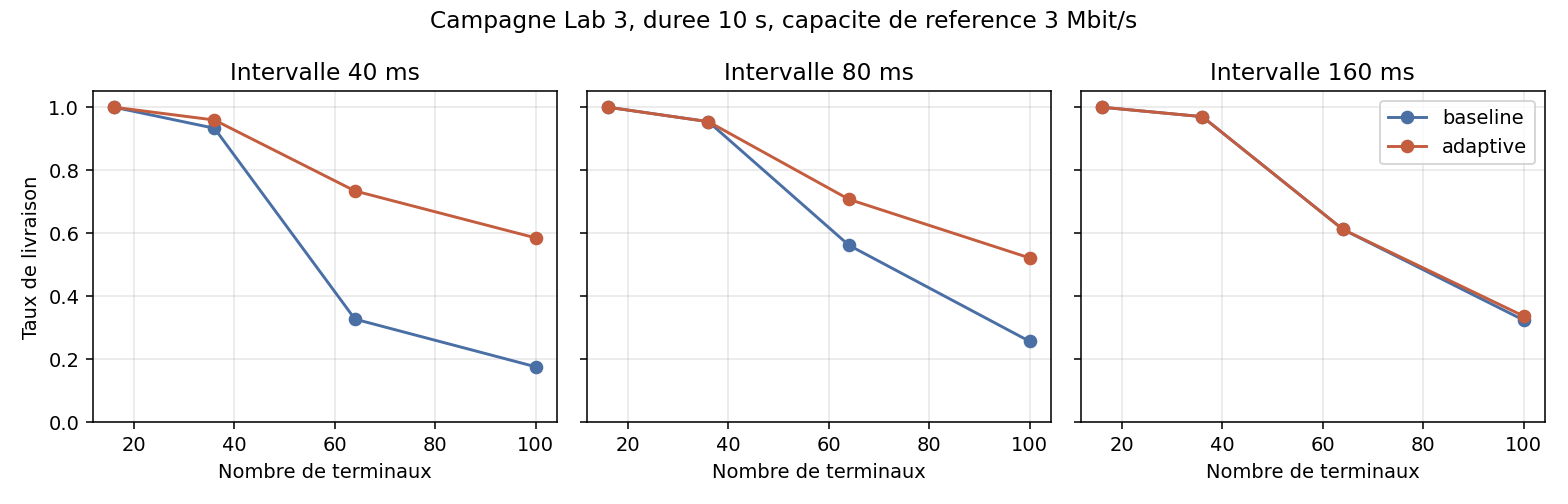
\includegraphics[width=\linewidth]{../../labs/lab03_controleur/sorties/livraison_campagne.png}
  \caption{Taux de livraison des octets réellement émis, selon le nombre de terminaux et l'intervalle. Les courbes se séparent lorsque $K$ est inférieur au nombre de terminaux.}
\end{figure}

\begin{figure}[H]
  \centering
  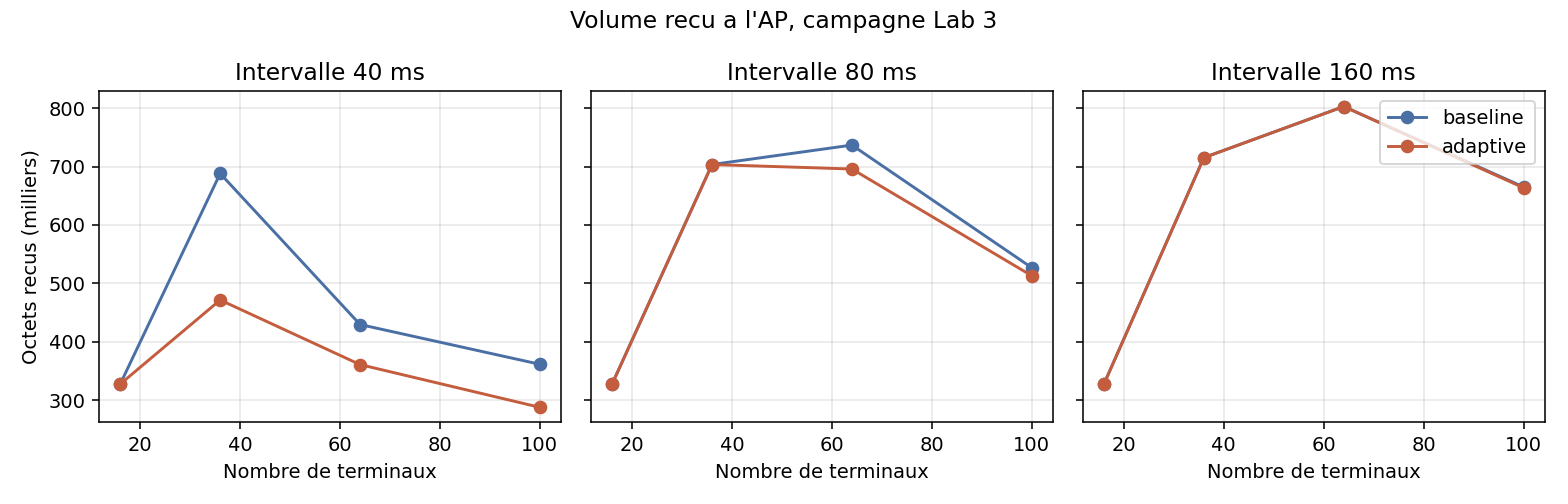
\includegraphics[width=\linewidth]{../../labs/lab03_controleur/sorties/octets_campagne.png}
  \caption{Octets reçus par le point d'accès. Lorsque l'admission retire des terminaux, le volume agrégé diminue, y compris dans les cellules où le taux de livraison augmente.}
\end{figure}

\begin{figure}[H]
  \centering
  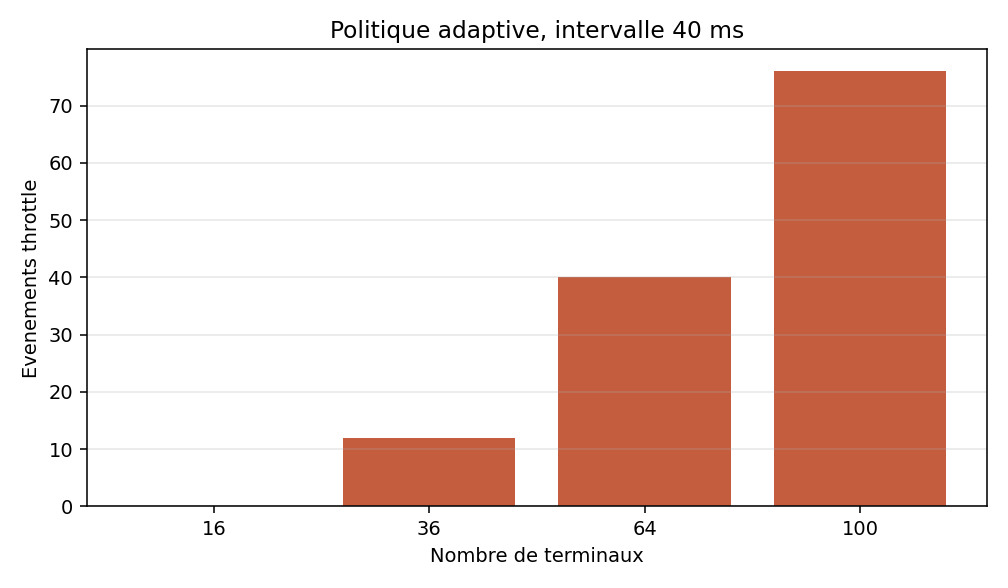
\includegraphics[width=0.72\linewidth]{../../labs/lab03_controleur/sorties/throttle_40ms.png}
  \caption{Événements de la politique adaptive à 40~ms. Le compteur vaut 0, 12, 40 et 76 pour 16, 36, 64 et 100 terminaux, ce qui est exactement le nombre de terminaux au-delà de $K = 24$.}
\end{figure}

\section{Interprétation}

Sur 16 terminaux, $K$ dépasse la taille de la grille pour les trois intervalles. La livraison vaut 1, l'indice de Jain vaut 1, et les deux politiques reçoivent 327\,680 octets. Ce volume est identique à celui du Lab 2. Le nouvel émetteur ne change donc pas le service lorsque le canal absorbe tout le budget.

Sur 36 terminaux, l'admission n'agit qu'à 40~ms. Le taux passe de 0,933 à 0,959, et les octets reçus passent de 688\,128 à 471\,552, soit une baisse d'environ 31~\%. Douze terminaux sont exclus, et FlowMonitor ne suit plus que 24 flux, ce qui confirme que les terminaux silencieux n'émettent rien. À 80~ms et à 160~ms, les deux politiques coïncident. La livraison baseline vaut 0,954 puis 0,970.

Sur 64 terminaux, l'intervalle de 40~ms est le cas le plus contrasté de cette grille. La baseline livre 0,328 des octets émis et reçoit 429\,568 octets. L'admission, limitée à 24 terminaux, livre 0,734 des octets émis et reçoit 360\,960 octets. Le taux augmente d'environ 0,41, tandis que le volume reçu baisse d'environ 16~\%. À 80~ms, $K$ vaut 48. Le taux passe de 0,562 à 0,708, et le volume passe de 736\,768 à 695\,808 octets, soit une baisse d'environ 5,6~\%. À 160~ms, $K$ vaut 96, les deux politiques reçoivent 802\,816 octets, et le taux vaut 0,613.

Sur 100 terminaux, la baseline reçoit 361\,472 octets à 40~ms, 526\,848 octets à 80~ms et 665\,088 octets à 160~ms. Les taux correspondants valent 0,177, 0,257 et 0,325. L'admission à 40~ms ne garde que 24 terminaux. Le taux monte à 0,585, et le volume tombe à 287\,744 octets, soit une baisse d'environ 20~\%. À 80~ms, 48 terminaux restent admis. Le taux passe de 0,257 à 0,522, et le volume passe de 526\,848 à 513\,024 octets, soit une baisse d'environ 2,6~\%. À 160~ms, seuls 4 terminaux sont exclus. Le taux passe de 0,325 à 0,338, et le volume passe de 665\,088 à 663\,552 octets. L'effet devient alors marginal, ce qui est cohérent avec un plafond de 96 terminaux sur une grille de 100.

L'indice de Jain publié est calculé sur les flux dont le nombre d'octets reçus est strictement positif. Les terminaux réduits au silence n'y entrent pas. À 100 terminaux et 40~ms, l'indice adaptive de 0,838 décrit l'équité entre les 24 flux admis, alors que l'indice baseline de 0,918 décrit l'équité entre 100 flux qui ont tous reçu au moins un octet. Une équité calculée sur la population entière, avec des zéros pour les stations exclues, serait plus basse pour la politique adaptive. Le tableau ne fournit pas ce second indice, parce que le CSV ne conserve pas le détail par flux.

Le gain défendable porte donc sur la fraction des octets émis qui arrivent au point d'accès, et sur la disparition des collisions dues aux terminaux exclus. Le volume agrégé reçu diminue dans chacune des six cellules où l'admission retire au moins un terminal. Le contrôleur protège un sous-ensemble. Il n'augmente pas le service total de la cellule sur ce proxy Wi-Fi.

\section{Écart avec le CSV du Lab 2}

Le CSV du Lab 2 a été produit avec \texttt{UdpClient}. Le source actuel le remplace par les sockets planifiés dans \texttt{SendSta}, et le premier paquet de chaque terminal est décalé d'une fraction d'intervalle. D'autres différences de pile, entre \texttt{UdpClient} et un socket UDP nu, peuvent aussi contribuer. La campagne ne sépare pas ces effets.

Les baselines coïncident à 16 terminaux, avec 327\,680 octets. Elles s'écartent lorsque la grille sature. À 100 terminaux et 40~ms, le Lab 2 recevait 381\,440 octets et le Lab 3 en reçoit 361\,472. L'écart le plus net concerne 64 terminaux à 40~ms, où le Lab 2 recevait 572\,928 octets et le Lab 3 en reçoit 429\,568. Les deux CSV ne doivent pas être fusionnés. Relancer le script du Lab 2 avec le source actuel écraserait l'archive \texttt{UdpClient} et ne reproduirait pas le rapport du Lab 2.

\section{Limites}

La campagne repose sur une seule graine. Les petits écarts, en particulier celui de 100 terminaux à 160~ms, ne soutiennent pas une affirmation statistique. Une répétition avec plusieurs \texttt{RngRun} reste nécessaire avant de conclure sur un écart de quelques millièmes.

La capacité de 3~Mbit/s est un paramètre de la loi, et non une mesure du canal \texttt{HtMcs7}. Changer cette capacité change $K$, donc change l'ensemble des cellules où les politiques se séparent. Le résultat est conditionnel à ce choix, qui a été fixé pour que l'admission soit visible sur le plan du Lab 2.

L'admission suit l'indice de création des terminaux. Elle ne tient pas compte de la position dans la grille ni du rapport signal sur interférence. Deux terminaux de même indice relatif seraient traités de la même façon dans une autre géométrie. Enfin, le proxy reste du Wi-Fi 802.11n. Les chiffres ne sont pas des indicateurs IMT-2030 de connectivité massive à l'échelle du kilomètre carré.

\section{Conséquence pour la suite}

Le Lab 3 atteint l'objectif laissé ouvert par le Lab 2. La politique adaptive modifie désormais une métrique de service, et le mécanisme est visible dans le CSV, puisque le nombre de flux suivis égale $K$ dès que le plafond est contraignant. Le prix de cette modification est une baisse du volume reçu. Un contrôleur ultérieur qui viserait le volume agrégé devra donc chercher une autre loi, par exemple une admission plus large, ou une répartition dans le temps qui conserve davantage d'émetteurs sans revenir à la collision de la baseline.

Le Lab 4 constate que le module NR est absent de cet arbre ns-3.43, et il ne publie donc aucun chiffre NR. Le Lab 5 reprend la même radio et remplace le plafond fixe par une boucle qui observe la livraison de la fenêtre courante. Le présent rapport reste la référence de l'admission fixe, avec la distinction maintenue entre taux de livraison des octets émis et volume reçu par le point de collecte.

\section{Reproduction}

\begin{lstlisting}[language=bash]
cd /mnt/c/Users/MOH/Documents/Projet_Perso/ns-allinone-3.43
python3 projet-visuel-imt2030/labs/lab03_controleur/scripts/lancer_campagne.py
python3 projet-visuel-imt2030/labs/lab03_controleur/scripts/analyser_campagne.py
cd projet-visuel-imt2030/docs/latex
pdflatex rapport_lab03.tex
pdflatex rapport_lab03.tex
\end{lstlisting}

Le premier script suppose que le scénario du Lab 1 a déjà été copié dans le scratch. Il relance la compilation si ce source a changé. Le CSV historique du Lab 2 doit être conservé à part.

\end{document}
